%-------------------------------------------------------------------------------
%	DIRC TECHNOLOGY CHAPTER
%-------------------------------------------------------------------------------
\label{ch:components}
The validation of key components of the DIRC for an EIC in vital to show that the Geant4 simulation package produces results expected for the real detector. However, due to budget restraints it was not possible to build or otherwise procure a full scale prototype of the envisioned EIC DIRC discussed in Chapter \ref{ch:eicdirc} (e.g. $2\unit{mm}$ pixel MCP-PMTs are not available on the market). Instead a series of test bench measurements were made for both the NLaK33 material of the 3-layer lens and for the performance of similar MCP-PMTs in high magnetic field environments.

\begin{figure}[ht]
	\centering
	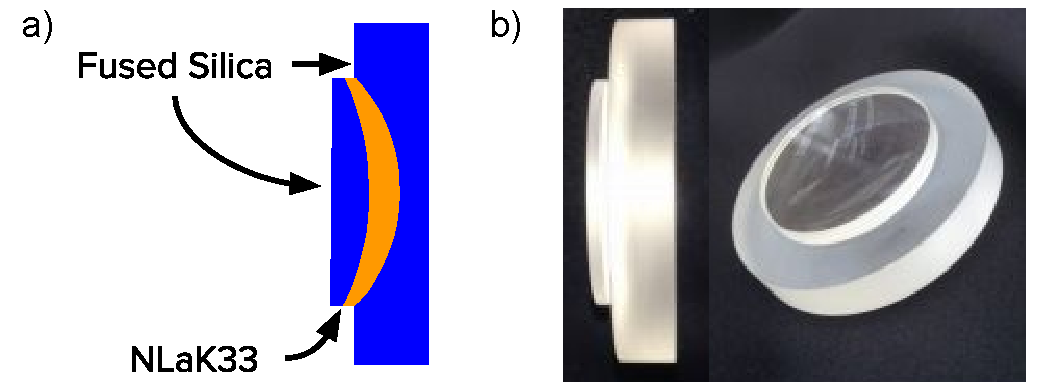
\includegraphics[width=\textwidth]{3CS_schematic.pdf}
	\caption{Schematic drawing of the 3-layer lens design with two layers of fused silica sandwiching a layer of high refractive index NLaK33 glass (a), and a side and front view of a prototype lens built for testing (b).}
	\label{fig:3CS_schematic}
\end{figure}



%-------------------------------------------------------------------------------
%	3-LAYER LENS OPTICS SECTION
%-------------------------------------------------------------------------------
\section{Optical Properties of 3-Layer Lens}
The FDIRC R\&D program first developed the concept of using focusing mirrors for DIRC detectors. The PANDA Barrel DIRC group settled on using a focusing lens between the radiator bar and the expansion volume. A standard lens made of fused silica with an air gap between the lens and the expansion volume was first studied. Figure \ref{fig:airgap_dispersion} shows that while this air gap lens provides good focusing of the Cherenkov pattern in the central region of the ring, it becomes defocused nearer to the edges of the pattern and loses photons due to either internal reflections in the lens due to the jump in index of refraction, or from photons at steeper angles exiting the lens and missing the expansion volume entirely.

\begin{figure}[ht]
	\centering
	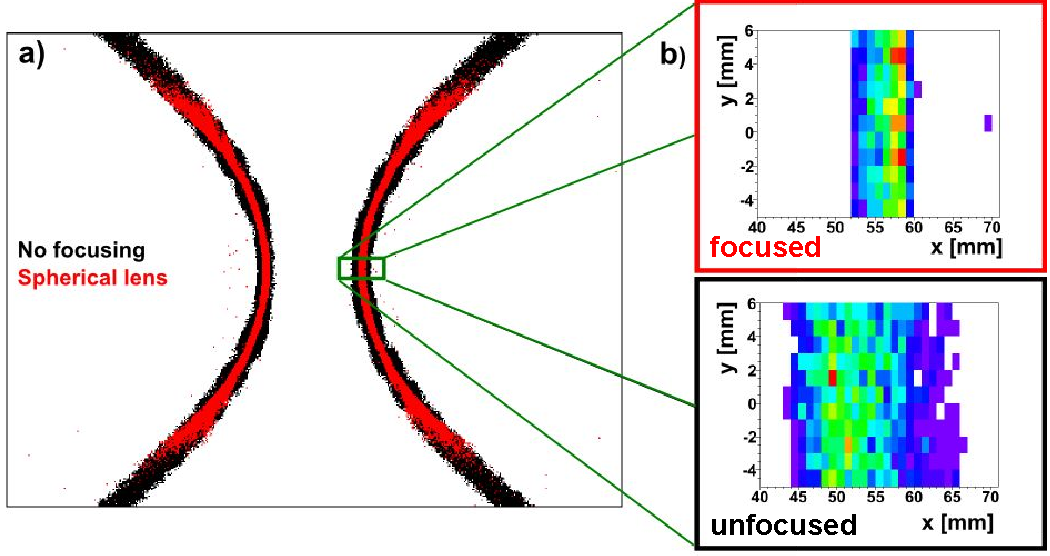
\includegraphics[width=\textwidth]{airgap_dispersion.pdf}
	\caption{Simulated hit pattern of PANDA DIRC without (black) and with (red) air gap lens focusing (a). On the outer edges of the ring image the lens is becoming dispersive  and losing photons, while near the center of the rings the lens does a good job of focusing the image, as seen more clearly in b).}
	\label{fig:airgap_dispersion}
\end{figure}

Next a 2-layer lens

The advantage of this 3-layer lens design over a traditional optical lens or a 2-layer lens is the shape of the focal plane. According to simulation the focal plane of the 3-layer lens is relatively flat, as shown in Figure \ref{fig:lens_focal_plane}. 

\begin{figure}[ht]
	\centering
	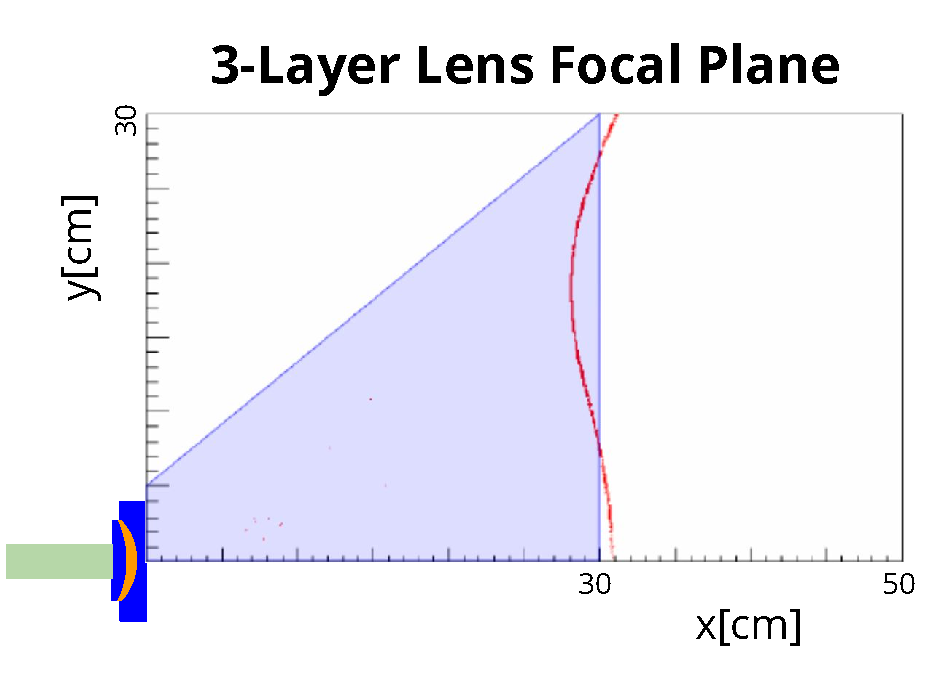
\includegraphics[width=0.5\textwidth]{3CS_focalplane.pdf}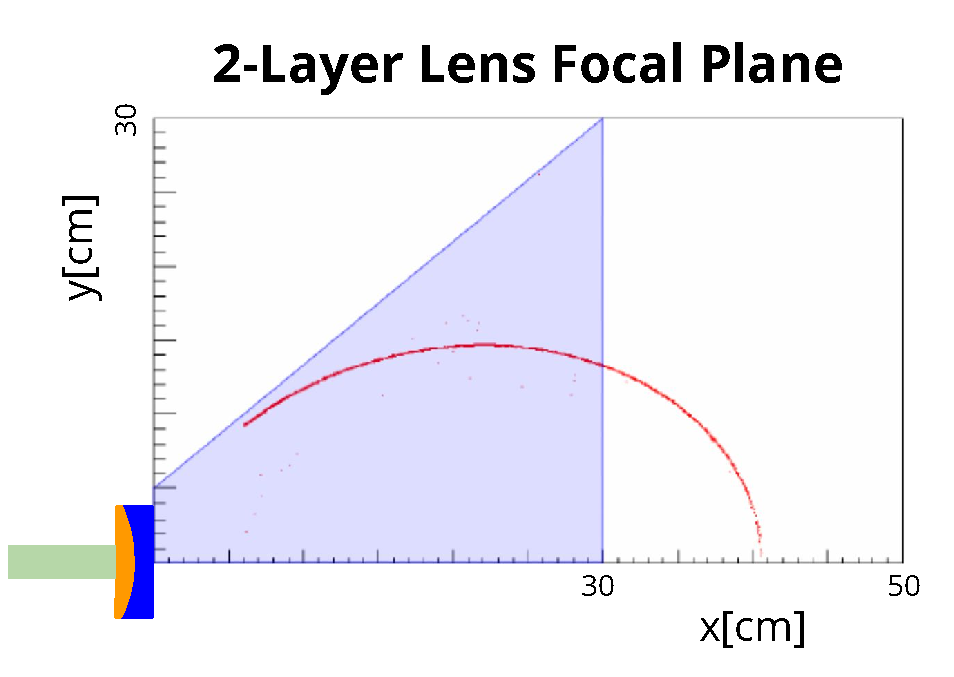
\includegraphics[width=0.5\textwidth]{2CS_focalplane.pdf}
	\caption{The simulated focal planes (red lines) of the 3-layer lens (left) and a 2-layer lens (right) compared to the shape of the expansion volume prism (grey). Obviously the focal plane of the 2-layer lens is highly parabolic in shape, whereas the 3-layer lens focal plane is relatively flat, allowing for a better resolution of the Cherenkov angle.}
	\label{fig:lens_focal_plane}
\end{figure}

%-------------------------------------------------------------------------------
%	NLAK33 RAD HARDNESS SECTION
%-------------------------------------------------------------------------------
\section{Radiation Hardness of NLaK33 Material}

%-------------------------------------------------------------------------------
%	HIGH-B TESTS SECTION
%-------------------------------------------------------------------------------
\section{Performance of MCP-PMTs in High Magnetic Field}